\documentclass[border=10pt]{standalone}
\usepackage{tikz}
\usetikzlibrary{shapes.geometric, arrows.meta, positioning}

% Define flowchart styles
\tikzstyle{startstop} = [
    rectangle, 
    rounded corners, 
    minimum width=3cm, 
    minimum height=1cm,
    text centered, 
    draw=black, 
    fill=red!30,
    font=\bfseries
]

\tikzstyle{io} = [
    trapezium, 
    trapezium left angle=70, 
    trapezium right angle=110, 
    minimum width=3cm, 
    minimum height=1cm, 
    text centered, 
    draw=black, 
    fill=blue!30
]

\tikzstyle{process} = [
    rectangle, 
    minimum width=3cm, 
    minimum height=1cm, 
    text centered, 
    draw=black, 
    fill=orange!30
]

\tikzstyle{decision} = [
    diamond, 
    minimum width=3cm, 
    minimum height=1cm, 
    text centered, 
    draw=black, 
    fill=green!30,
    aspect=2
]

\tikzstyle{arrow} = [thick,->,>=Stealth]

\begin{document}

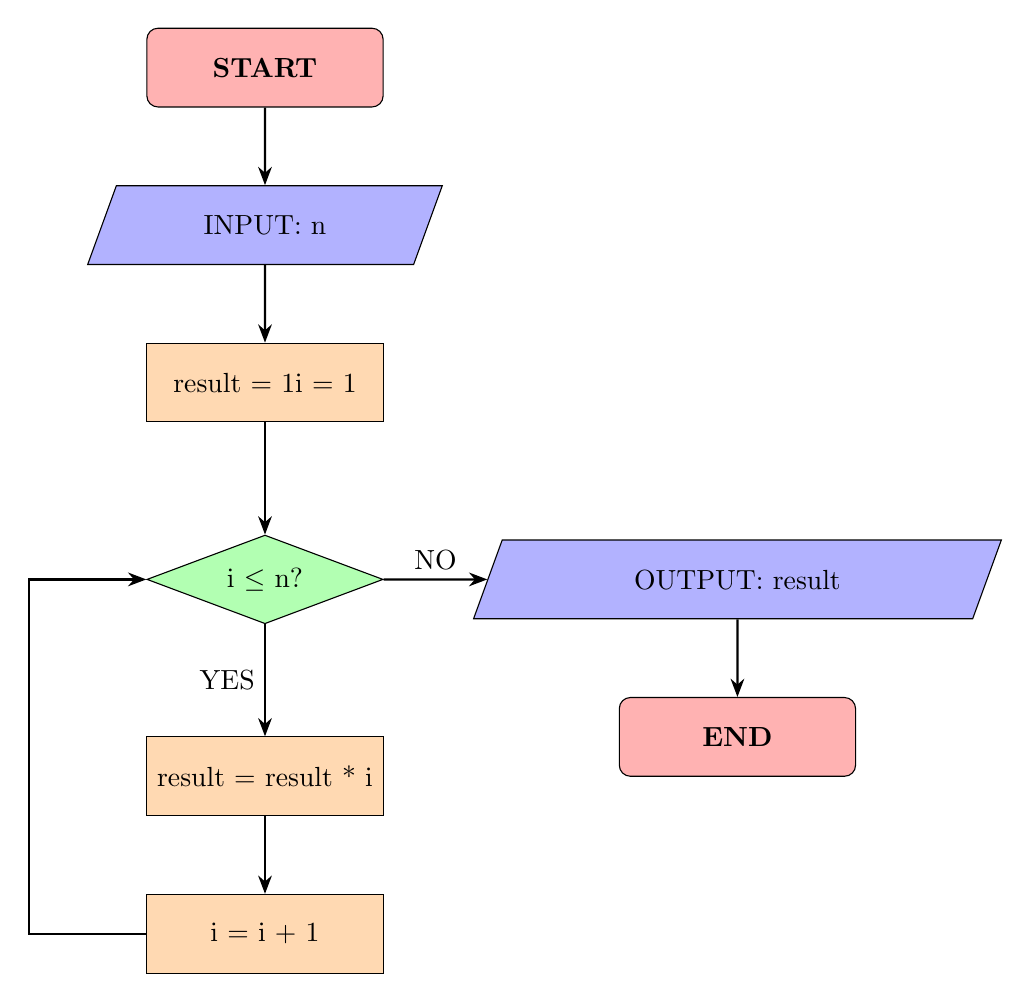
\begin{tikzpicture}[node distance=2cm]

% Nodes
\node (start) [startstop] {START};
\node (input) [io, below of=start] {INPUT: n};
\node (init) [process, below of=input] {result = 1\\ i = 1};
\node (decision) [decision, below of=init, yshift=-0.5cm] {i \(\leq\) n?};
\node (multiply) [process, below of=decision, yshift=-0.5cm] {result = result * i};
\node (increment) [process, below of=multiply] {i = i + 1};
\node (output) [io, right of=decision, xshift=4cm] {OUTPUT: result};
\node (end) [startstop, below of=output] {END};

% Arrows
\draw [arrow] (start) -- (input);
\draw [arrow] (input) -- (init);
\draw [arrow] (init) -- (decision);
\draw [arrow] (decision) -- node[anchor=east] {YES} (multiply);
\draw [arrow] (multiply) -- (increment);
\draw [arrow] (increment) -- +(-3,0) |- (decision);
\draw [arrow] (decision) -- node[anchor=south] {NO} (output);
\draw [arrow] (output) -- (end);

\end{tikzpicture}

\end{document}
